\documentclass{sig-alternate}

\usepackage{url}

\begin{document}
%
% --- Author Metadata here ---
%\conferenceinfo{Potentially Systems Research}{'14 Pompeii, Italy}
%\CopyrightYear{2007} % Allows default copyright year (20XX) to be over-ridden - IF NEED BE.
%\crdata{0-12345-67-8/90/01}  % Allows default copyright data (0-89791-88-6/97/05) to be over-ridden - IF NEED BE.
% --- End of Author Metadata ---

\title{Amdahl's Ratios: The Balancing of Power for Large Data Centers}

\numberofauthors{2} %  in this sample file, there are a *total*
% of EIGHT authors. SIX appear on the 'first-page' (for formatting
% reasons) and the remaining two appear in the \additionalauthors section.
%
\author{
% You can go ahead and credit any number of authors here,
% e.g. one 'row of three' or two rows (consisting of one row of three
% and a second row of one, two or three).
%
% The command \alignauthor (no curly braces needed) should
% precede each author name, affiliation/snail-mail address and
% e-mail address. Additionally, tag each line of
% affiliation/address with \affaddr, and tag the
% e-mail address with \email.
%
% 1st. author
\alignauthor
Vincent Lee\\
       \affaddr{Department of Computer Science and Engineering}\\
       \affaddr{University of Washington}\\
       \affaddr{Seattle, Washington}\\
       \email{vlee2@cs.washington.edu}
% 2nd. author
\alignauthor
Shumo Chu\\
       \affaddr{Department of Computer Science and Engineering}\\
       \affaddr{University of Washington}\\
       \affaddr{Seattle, Washington}\\
       \email{chushumo@cs.washington.edu}
% 3rd. author
% \alignauthor NULL POINTER\\
%       \affaddr{The Ivory Tower}\\
%       \affaddr{Institute of Exascale Computing}\\
%       \affaddr{Atlantis, Hawaii}\\
%       \email{SEGFAULT@atlantis.gg}
}
\date{5 December 2014}

\maketitle
\begin{abstract}

The advent of large distributed systems has enabled unprecedented amounts of computational resources to the end user.
Large data centers today use enormous numbers of commodity servers and routers to operate over massive data sets.
Due to the massive scale of deployment, small software and hardware architectural changes that influence power, network bandwidth, and memory efficiency have enormous impact.
With the rise of big data applications, and dynamically shifting workload patterns, it is imperative that we understand how production workloads on these systems behave in order to determine what aspects of the system architecture work well and what should be changed.
In particular, we explore whether the Amdahl's Rules of Thumb for a balanced system still hold for today's data center applications or if they are shifting to meet the demands of these systems.
We analyze the Google Cluster Trace to extrapolate order of magnitude estimates as to whether these system ratios between compute, memory, and disk still hold.

\end{abstract}

% A category with the (minimum) three required fields
%\category{H.4}{Information Systems Applications}{Miscellaneous}
%A category including the fourth, optional field follows...
%\category{D.2.8}{Software Engineering}{Metrics}[complexity measures, performance measures]

\terms{distributed systems}

\keywords{distributed systems, data center, workload analysis}

\section{Introduction}

System designs today are driven by a myriad of factors such as application workload, performance targets, energy efficiency constraints, and system scalability.
To build these systems, we rely largely on empirical analyses of application workloads and intuition to properly engineer the amount of computation, memory, disk, and networking I/O to satisfy the resource requirements or constraints of the system.
To quantify the relationship between each of these system components, we build ratios between the amount of compute, memory, disk, and networking I/O; we collectively refer to these ratios as the ``system balance''.
Ideally we'd like to construct systems which have sufficient amounts of memory, compute, disk, and network I/O but are not over-provisioned.
A system with insufficient resources can result in poor performance as a single component of the system can bottleneck progress.
Alternatively, a system with over-provisioned resources is wasteful and can expend unnecessary energy and silicon.

%We term such a system which is sufficient resources and not over-provisioned as a ``balanced system'' and the ratios between compute, memory, disk, and IO the ``system balance''.

Amdahl's Law first proposed in ~\cite{Amdahl:1967:VSP:1465482.1465560} outlines some of the first known system balance rules; most notably Amdahl's parallelism law.
However, subsequent interpretations and reevaluations of Gene Amdahl's original work have derived additional relationships between system components as described in ~\cite{Gustafson:1988:RAL:42411.42415, Hill:2008:ALM:1449375.1449387, export:68636, Bell:2006:PCS:1110638.1110681}.
These relationships have become known as ``Amdahl's Rules of Thumb'' and seek to quantify the ideal system balance configurations.

For decades, Amdahl's Rules of Thumb have continued to hold despite rapid scaling in silicon, memory, and networking technology.
As outlined by J. Gray et. al. ~\cite{export:68636}, the original Amdahl's Rules of Thumb for a balanced system consist of:
\begin{enumerate}
\item Amdahl's parallelism law: if a computation has serial component S and parallel component P, then the maximum speedup is (S+P)/S
\item Amdahl's balanced system law: a system needs one bit of memory IO per second for each instruction per second
\item Amdahl's memory law: in a balanced system, the ratio $\alpha$ of the size of memory in MB to the instructions per second in million instructions per second (MIPS) is 1 MB per 1 MIPS or $\alpha = 1$
\item Amdahl's IO law: programs do one memory IO per 50000 instructions
\end{enumerate}
However, the advent of large scale distributed computing and data centric applications has drastically changed the landscape of computing platforms and the methods we employ when engineering systems.
Such systems may consist of millions of homogeneous cluster nodes or a heteogeneous spread of specialized hardware such as GPUs and custom accelerators.
Cluster nodes may entirely be dedicated to serve as storage nodes or compute nodes, and cluster resource usage may be mediated by a centralized scheduler.
In these large, dynamic, and potentially heterogeneous data center landscapes, it is unclear whether systems we build today are still considered balanced systems under Amdahl's Rules of Thumb.

Using the Google cluster data set ~\cite{clusterdata:Wilkes2011, clusterdata:Reiss2011}, we attempt to extrapolate a more current picture of how the ratios between computation, memory, and disk behave today in data centers.
The Google cluster data set contains details about usage statistics for individual tasks scheduled on a Google cluster over a period of roughly a month in 2011.
In particular we compare the ratios between requested compute, memory, and disk resources, and actual compute, memory, and disk usage for each task scheduled in the cluster.
The ratio between requested resource sizes allow us to estimate what resources the application programmers and scheduler think a required from the system.
A comparison with actual usages will allow us to view whether request ratios are fully accurate in addition to validating whether Amdahl's Rules of Thumb for a balanced system still hold.

\section{Google Cluster Data}

The Google cluster data contains a total of 6 different traces:
\begin{enumerate}
\item Job Events: record of the state changes to each job running on the system
\item Task Usage: task resource usage such as memory, CPU rate, and disk for each task
\item Machine Attributes: defines properties and configurations for each machine
\item Machine Events: trace of when machines are added, removed, or updated
\item Task Constraints: lists the placement constraints for various tasks
\item Task Events: lists attributes about the scheduled tasks such as number of requested resources, job priority, and scheduling class
\end{enumerate}
We use Myria \cite{HalperinACCKMORWWXBHS14SIGMOD} as our data analytics platform to analyze the Task Usage and Task Events traces to extract the resource usage ratios.

\subsection{Cleaning Known Trace Anamolies}

While a vast majority of data set fields are complete entries, the original creators note several anamolies in the trace attributed to profiler bugs or profiler overload.
Most of these anamolies are missing data fields which occur in less than 0.1\% of the data set entries.
However, there is a significant omission is the disk-time fraction measurement in the Task Events trace due to ``a change in [their] monitoring system'' which results in 15 days out of the 29 days missing this field.
Since Myria requires a clean dataset with no missing fields, we ran a script to clean up each part of the trace.
For missing numerical fields, we insert a value of -1 into the trace.
Since all numerical values in the trace are positive floating points or integers, when performing our analysis we siplmy skip over fields which are -1.
For missing boolean fields, we assume arbitrarily by default the presence of the attribute is false.
This does not affect our results as we do not perform any queries over these boolean fields.

\subsection{Obfuscated Data Calculations}

Most fields in the trace have been obfuscated; for instance, the size of memory that may be requested is normalized to be a fraction of the largest memory unit available in the system as opposed to the absolute amount of memory requested in bytes.
If it becomes necessary in our calculations to use the actual memory size in bytes, we attempt to use reasonable order of magnitude values.
In the above case we might assume one unit worth of memory may be 1 or 2 GB.
As far as we can tell, CPU rate, memory, disk space, and disk time fraction are all affected by this normalization technique.

\section{High Level Statistics}

\subsection{Machine Events}

The machine\_events table consists of entries which record when machines are added, removed, or updated in the cluster.
Each record contains the CPU resource capacity and memory capacity normalized out of the largest of each respective capacity.
Each record also contains an obfuscated hash of the platform or hardware used for each machine.

We quickly analyze the distribution of Platform IDs as it provides a picture of the homogeneity of the hardware platforms.
Each Platform ID hash corresponds to one combination of hardware (CPU cores, memory, disk, etc.).
Figure ~\ref{platform_dist} shows the distribution of hardware platforms deployed in the cluster.
We arbitrarily map the nth obfuscated Platform ID field to Type n in Figure ~\ref{platform_dist} for simplicity.
Not surprisingly, we find that cluster is overwhelmingly composed of a single platform indicating a fairly homogeneous system.
We suspect the minority of machines are specially equipped platforms that may be used for specially contrained tasks.

\begin{figure}
\centering
\begin{tabular}{| c | c |} \hline
Platform Type & Number of Machines\\ \hline
Type 1 & 798\\ \hline
Type 2 & 126\\ \hline
Type 3 & 11659 \\ \hline
\end{tabular}
\label{platform_dist}
\caption{Number of Each Type of Hardware Platform Deployed in Cluster}
\end{figure}

%\subsection{Task Event Analysis}

%The task\_event trace tracks the resource request amounts in addition to task priorities.
%Of particular interest are the resource usage request amounts for CPU cores, RAM, and local disk space; again, these values were obfuscated by normalizing out of the maximum capacities of each resource.

%\begin{figure}
%\centering
%\begin{tabular}{| c | c | c | c |} \hline
%Resource Request & Avg & Min & Max \\ \hline
%CPU cores & & & \\ \hline
%RAM & & & \\ \hline
%Disk Space & & & \\ \hline
%\end{tabular}
%\label{resource_summary}
%\end{figure}

%\begin{figure}
%TODO: configuration histograms should go here for CPU
%\end{figure}

%\begin{figure}
%TODO: configuration histograms should go here for memory
%\end{figure}

%\begin{figure}
%TODO: configuration histograms should go here for ratio
%\end{figure}

%TODO: brief analysis

\subsection{Task Usage Analysis}

The task\_usage trace tracks the resource usage requests for each task executing on the cluster.
Each entry in the trace reflects values sampled over 300 seconds of the task or the entire task duration, which ever time span is shorter.
Of particular interest in this trace are the average and peak usages for CPU, memory, and local disk, and the ratios between these qualitities.
We also analyze the cycles per instruction (CPI), and memory accesses per instruction (MAI).
Figure ~\ref{task_usage_stats} shows the average, minimum value, and maximum value for each of the fields of interest; note again that some fields are normalized out of the maximum value seen in the trace.
For many of these fields however, we expect that the normalization factors are very close to or on the same order of magnitude as their resource capacities as the distributions are heavily tailed.

\begin{figure}
\centering
\begin{tabular}{| p{2.5cm} | p{1.5cm} | p{1.5cm} | p{1.5cm} |} \hline
 & Avg & Min & Max \\ \hline
Avg CPU Usage & 0.023 & 0 & 145.8 \\ \hline
Avg Memory Usage & 0.023 & 0 & 0.881 \\ \hline
Avg Local Disk Space & 0.000125 & 0 & 0.00726 \\ \hline
Assigned Memory & 0.029 & 0.00000477 & 229100\* \\ \hline
Peak Memory Usage & 0.024 & 0 & 0.886 \\ \hline
Disk I/O Time & 0.00357 & 0 & 0.685 \\ \hline
Peak CPU Rate & 0.0904 & 0 & 1744\* \\ \hline
Peak Disk I/O Time & 0.0232 & 0 & 10.98 \\ \hline
CPI & 4.866 & 0 & 25370\* \\ \hline
MAI & 0.0176 & 0 & 8.5\* \\ \hline
\end{tabular}
\caption{Task Usage Trace Statistics - average, minimum, and maximum values for each quantity of interest}
\label{task_usage_stats}
\end{figure}

For certain fields marked with an \*, we see that the maximum values are greater than 1 and are sometimes unreaonably large.
Some of this decrepancy can be attributed to the way the profiling infrastructure aggregates statistics from subcontainers when the parent task container cannot be profiled.
As a result, the aggregation of the statistics which simply sums up individual subtask statistics can yield values greater than 1.
Some of the more unreasonable values are most likely attributed to errors in the way statistics were collected or bugs in the collection infrastructure.
For instance, the CPI measurement of 25370 is clearly not a reasonable data point and should hence be discarded.

Of particular interest, is the average MAI value.
This measurement reflects the performance counter value and to our knowledge is not normalized.
When compared to Amdahl's IO Law, the MAI indicates that on average one memory access occurs for every 56.8 instructions.
This is in stark contrast to the one memory access per 50000 instructions contended by Amdahl's Rules of Thumb suggesting that the workloads on these clusters are much more memory centric or data intensive.

\section{System Balance Calculations}

To calculate whether the system is balanced or not, a few additional compensation factors must be considered due to obfuscation of the original data set.
Namely, to compute the system balance ratios we must compensate for the normalization operations over the original data.
This means we cannot obtain exact estimates of the system balance, instead we extrapolate order of magnitude calculations which, for comparing Amdahl's Rules of Thumb, are sufficient.

To allow us to compute reasonable order of magnitude estimates we define some assumptions about the hardware.
We do not know exactly the parameters of each hardware platform but we can make a fairly reasonable estimate based on commodity hardware trends at the time of the trace collection.
As shown in ~\cite{googlehw} from 2009 (the same year the trace was collected), it appears the server motherboard contained at least two dual or quad core CPUs (from the fans), 8 standard DIMM memory slots, and two Hitachi Deskstar hard drives.
If we assume each of the DIMM memory slots contains 1 or 2 GB of RAM, a typical server would have between 8 and 16 GB of maximum memory capacity.
A typical commodity disk capacity for the Hitachi Deskstar around the time the trace was collected was around 1 TB putting the disk capacity per server at around 2 TB.

We use these estimates to compute order of magnitude calculations for the system balance ratios for the requested resource qualitites and actual resource usages.
To get a an order of magnitude sense of the system balance ratios, each histogram uses a log scale for each bucket and thus shows the number of tasks that fall under each order of magnitude.

\subsection{Request System Balance Ratios}

We first compare the system balance ratios of the requested CPU, memory, and disk resources by computing the average value of each ratio, and histogramming over each entry in the task\_events trace.
We compute three ratios: (1) the ratio of requested CPU to requested memory (2), the ratio of requested CPU to requested, (3) the ratio of requested memory to requested disk.
We then unnormalize each ratio by multiplying by appropriate extrapolated resource values.

Figure ~\ref{req_cpu_mem} shows the histogram distributions for the ratio between the CPU resource request to memory resource request. 
To convert to instructions per GB of memory, we multiply ratio taken from the trace which is in normalized CPU cores per normalized memory by the following quantities: (1) 1 normalized memory/(8 GB), (2) 4 CPU cores/(normalized core), (3) 2 Gibi-instructions / (CPU core).  %, (4) $1 / cycles per instructions$. TO
This gives the quantity: \\
(requested normalized cores)/(requested normalized memories) * (1 normalized memory)/(8 GB) * (4 CPU cores)/(1 normalized core) * (2 G instructions)/(CPU core) = (8 Gibi-instructions) / (8 GB)

But since this conversion factor is the unity, it is the same histogram as the normalized histogram.
Thus Figure ~\ref{req_cpu_mem} reflects both the normalized ratios and estimated ratios in instructions per byte of memory.

\begin{figure}[t]
\centering
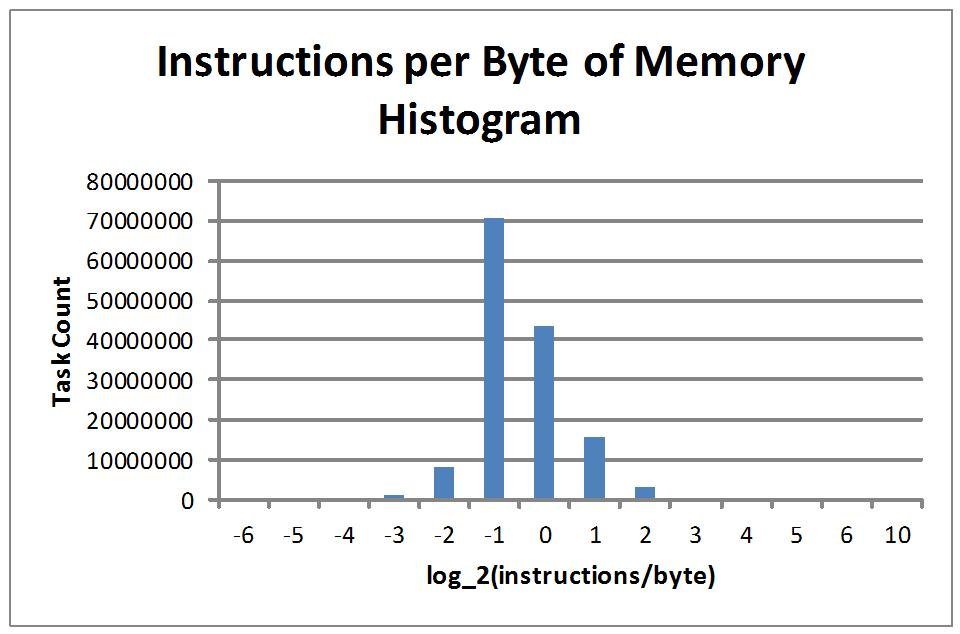
\includegraphics[width=3in]{../figures/req_cpu_mem.jpg}
\label{req_cpu_mem}
\caption{Histogram of normalized CPU resource request to memory request.}
\end{figure}

We perform a similar calculation with the ratio between the request for CPU cores and disk request size.
To convert to instructions per byte of disk space, we multiply by the following quantities: (1) 1 normalized disk/(1 TB), (2) 4 CPU cores/(normalized core), (3) 2 Gibi-instructions/(CPU core).
Figure ~\ref{req_cpu_disk} shows the histogram distributions for the ratio between the normalized CPU resource request and the normalized memory request.
Figure ~\ref{est_req_cpu_disk} reflects the histogram for the quantity calculated by: \\
(requested normalized cores)/(requested normalized disk) * (1 normalized disk)/(2 TB) * (4 CPU cores)/(1 normalized core) * (2 G instructions)/(CPU core) = 8 G instructions / 2 TB

\begin{figure}[t]
\centering
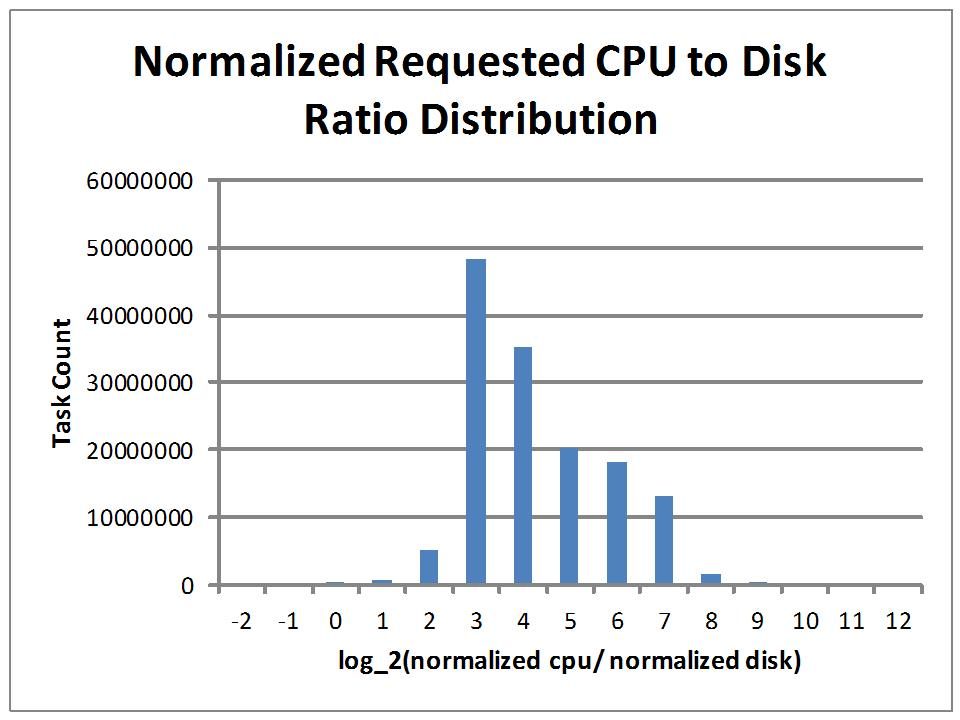
\includegraphics[width=3in]{../figures/req_cpu_disk.jpg}
\label{req_cpu_disk}
\caption{Histogram of normalized CPU resource request to disk request for all tasks.}
\end{figure}

\begin{figure}[t]
\centering
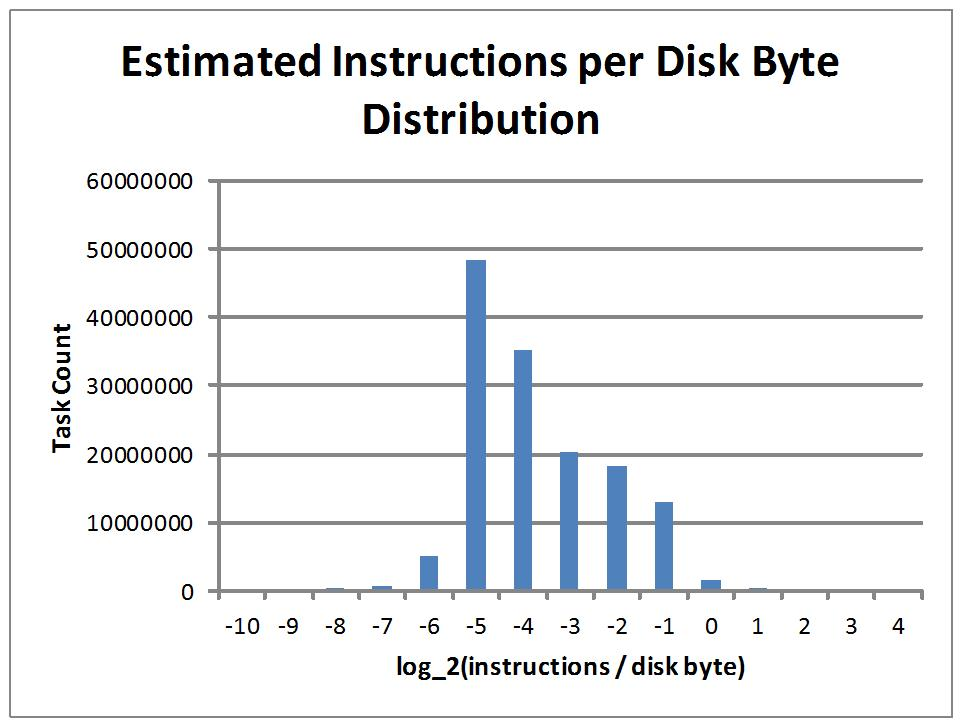
\includegraphics[width=3in]{../figures/est_req_cpu_disk.jpg}
\label{est_req_cpu_disk}
\caption{Histogram of estimated instructions per byte of disk for all tasks.}
\end{figure}

Finally, we compute the distribution of the ratio between normalized memory request and local disk request in Figure ~\ref{req_mem_disk}.
To obtain the estimate in bytes of memory per byte of disk, we multiply by the following conversion factors to the normalized memory request over normalized disk request: (1) 1 TB / 1 normalized disk (2) 1 normalized memory / 8 GB.
Figure ~\ref{est_req_mem_disk} histograms the resulting quantity:
(requested normalized memory)/(requested normalized disk) * (8 GB / normalized memory) * (1 normalized disk / 2 TB)

\begin{figure}[t]
\centering
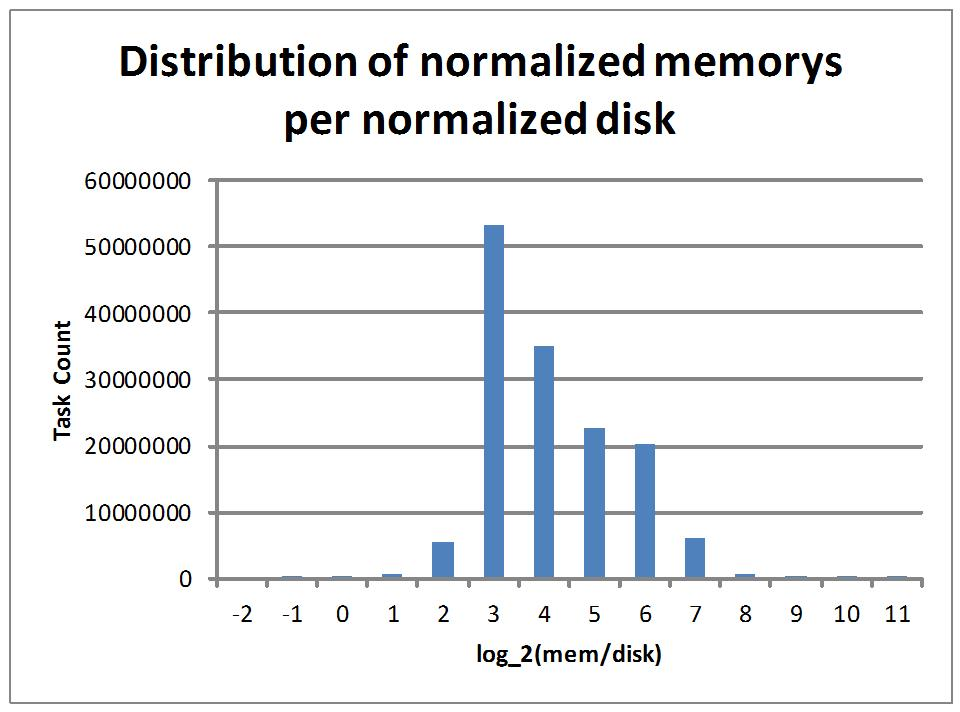
\includegraphics[width=3in]{../figures/req_mem_disk.jpg}
\label{req_mem_disk}
\caption{Histogram of normalized requested memories to disk request for all tasks.}
\end{figure}

\begin{figure}[t]
\centering
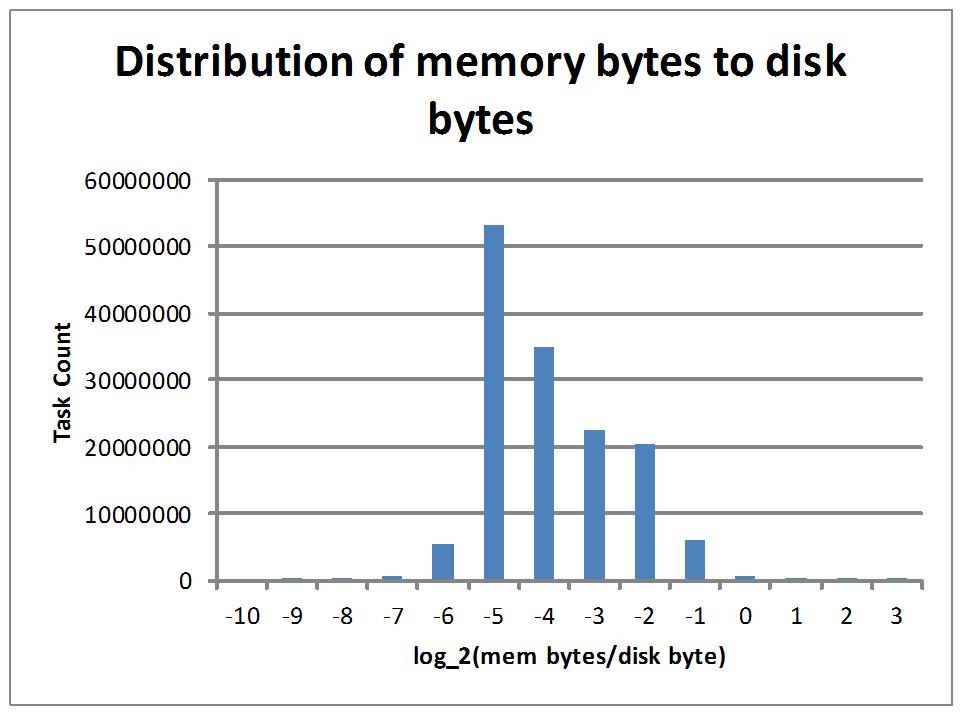
\includegraphics[width=3in]{../figures/est_req_mem_disk.jpg}
\label{est_req_mem_disk}
\caption{Histogram of estimated memory bytes per byte of disk for all tasks.}
\end{figure}

Figure ~\ref{request_summary} summarizes the resulting average value, minimum value, and maximum values observed in the resource request ratios.
We include an order of magnitude for the median values as Myria does not support a distributed median query calculation.
As a result, we use the histogram results to determine which order of magnitude the median value falls.
The statistics indicate that the distributions are heavily tailed and confirmed by the prior histogram data.
It is also interesting to note that the requested CPU to requested memory ratios are on the order of 1 instruction per byte of memory or $\alpha ~= 1$.
This suggests that Amdahl's memory law for system balance still appear to hold as far as resource request patterns go.

\begin{figure}
\centering
\begin{tabular}{| p{2cm} | p{1.25cm} | p{1.25cm} | p{1.25cm} | p{1.25cm } |} \hline
Ratio & Avg & Median & Min & Max \\ \hline
Req. CPU/Mem & 1.702 & $\approx 0.5$ & 0.00392 & 49160.986  \\ \hline
Est. Instr/Mem Byte & 1.702 & $\approx 0.5$ & 0.00392 & 49160.986 \\ \hline
Req. CPU/Disk & 403.730 & $\approx 16$ & 203208.556 & 0.184 \\ \hline
Est. Instr/Disk Byte & 1.577 & $\approx 0.0625$ & 793.783 & 0.000719 \\ \hline
Req. Mem/Disk & 260.060 & $\approx 16$ & 130334.487 & 0.200 \\ \hline
Est. Mem Byte/Disk Byte & 1.0159 & $\approx 0.0625$ & 509.119 & 0.000781 \\ \hline
\end{tabular}
\label{request_summary}
\caption{Summary of requested resource ratios}
\end{figure}

Another interesting statistic is that the estimate requested memory to local disk ratio is also on the order of 1 byte of memory per byte of request local disk.
This implies that most tasks seem to be optimized not to rely heavily on disk access operations as disk bandwidth can be crippling to applications.

\subsection{Actual System Balance Ratios}

We calculate the actual system balance ratios by taking the values from the task\_usage profile trace.
Like the resource request values in the task\_events trace, we apply transformations to the normalized data to get an estimate for the actual order of magnitude for each ratio.
Unlike the resource request ratios, task usage traces contain both an average usage and peak usage measurement for CPU and memory.
Furthermore, because trace values are normalized out of the largest value in the trace for each resource and not the large maximum capacity for each resource, we are limited to computing relative ratios using normalized values for each resource.

Figure ~\ref{avg_act_cpu_mem} shows the ratio between actual average CPU rate and average memory usage.

%Since trace values for actual usages are not normalized by maximum capacity but rather by the maximum value for the field that appears in the trace, we expect to see some deviations from the request ratios

\begin{figure}[t]
\centering
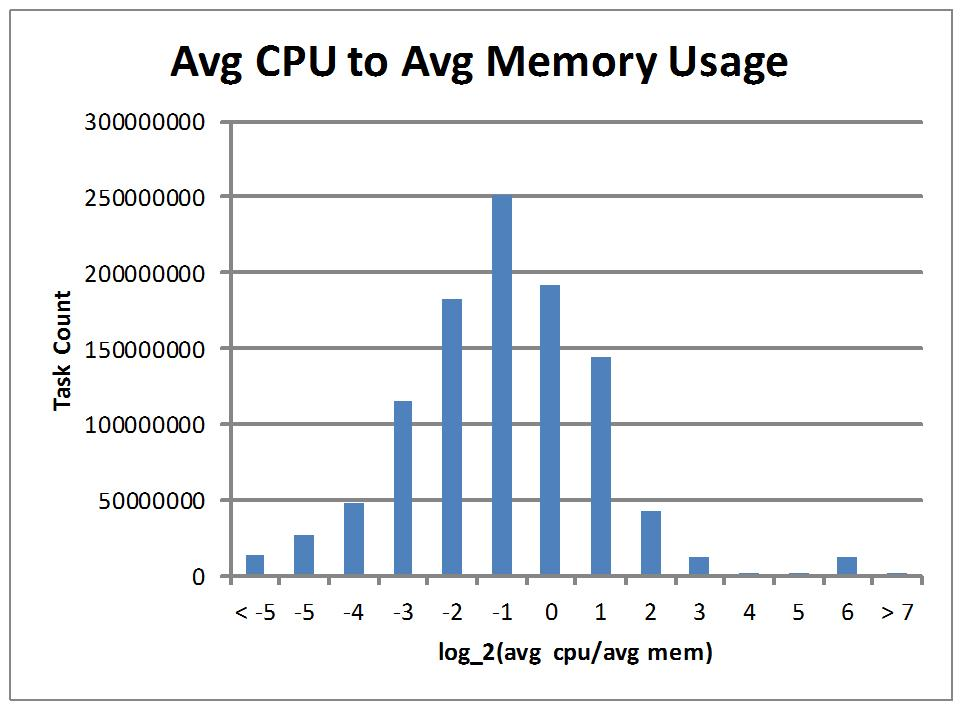
\includegraphics[width=3in]{../figures/avg_act_cpu_mem.jpg}
\label{avg_act_cpu_mem}
\caption{Histogram of ratio between normalized average CPU rate and normalized average memory usage over all tasks.}
\end{figure}

\begin{figure}[t]
\centering
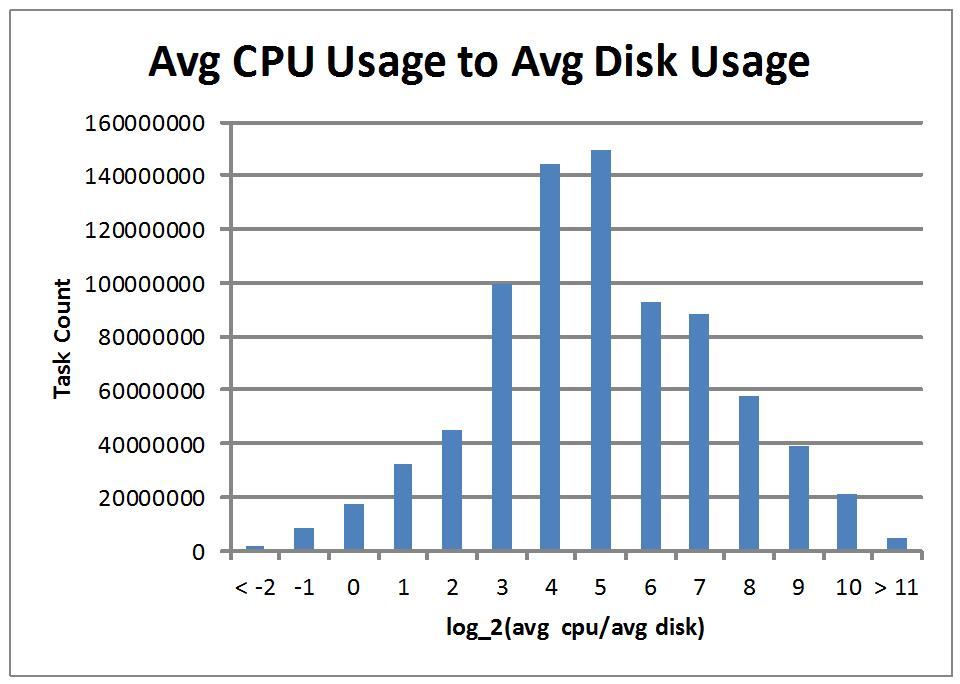
\includegraphics[width=3in]{../figures/avg_act_cpu_disk.jpg}
\label{avg_act_cpu_disk}
\caption{Histogram of ratio between normalized average CPU rate and normalized average local disk usage}
\end{figure}

\begin{figure}[t]
\centering
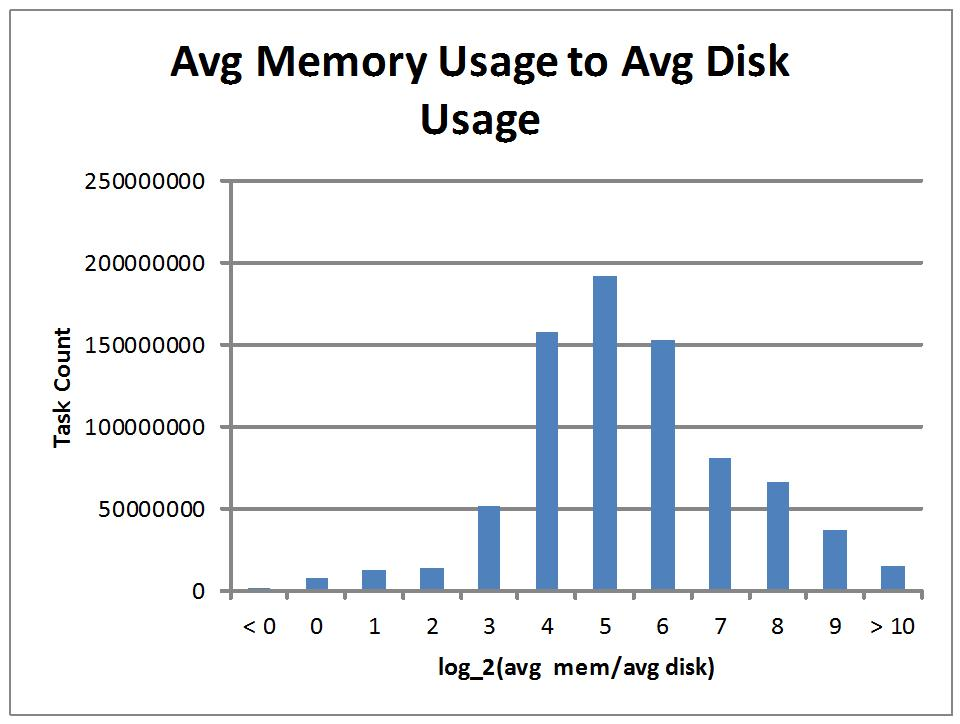
\includegraphics[width=3in]{../figures/avg_act_mem_disk.jpg}
\label{avg_act_mem_disk}
\caption{Histogram of ratio between normalized average memory usage and normalized average local disk usage}
\end{figure}

Figure ~\ref{actual_summary} shows the average value, minimum value, and maximum value for each of the ratios we compute in these usage histograms.
We also show the averages, minimum values, and maximum values for the average CPU to memory ratios, and average CPU to disk ratios adjusted for CPI.
By adjusting for CPI, this provides a closer metric to the true number of instructions executed per byte of memory or disk.
Similar to the resource request ratios, we see a heavily tailed distribution of each system balance ratio.

\begin{figure}[t]
\centering
\begin{tabular}{| p{2.5cm} | p{1.5cm} | p{1.5cm} | p{1.5cm} |} \hline
Ratio & Avg & Min & Max \\ \hline
Avg CPU/Avg Mem & 11.737 & 0.0000160 & 425920.100  \\ \hline
Avg CPU/Avg Disk & 2901.793 & 0.000263 & 152878263.605 \\ \hline
Avg Mem/Avg Disk & 2253.51 & 0.00102 & 579532.348 \\ \hline
Peak CPU/Peak Mem & 26.567 & 0.0000194 & 2008293.839 \\ \hline
Avg CPU/(Avg Mem * CPI) & 9.949 & 5.0193 & 293932.257 \\ \hline
Avg CPU/(Avg Disk * CPI) & 2443.536 & 0.00000522 & 66671724.206 \\ \hline
\end{tabular}
\label{actual_summary}
\caption{Summary of resource usage ratios}
\end{figure}

Of particular interest are the ratios between the CPU usage and memory usage.
In comparison with the normalized requested CPU and requested memory resources in ~\ref{request_summary}, these ratios appear to be an order of magnitude higher implying more computation per byte of memory is needed.
What is even more striking is when considering the ratio between peak CPU usage and peak memory usage, this ratio further increases.
While peak CPU operation does not usually correlate with peak memory usage, this shows further indicates that we should allocate more compute resources per byte of memory.

\section{Analysis}

\subsection{Amdahl's Parallelism Law}

Without question, Amdahl's Parallelism Law has continued the test of time. QED.

\subsection{Amdahl's Balanced System Law}

We cannot comment on this rule of thumb as the trace did not contain bandwidth measurements.

\subsection{Amdahl's Memory Law}

We observe that the estimated requested resource usage ratios mostly align with Amdahl's Memory Law which states the instruction per byte ratio $\alpha$ is around 1 or 1 MIPS per MB of memory.
As originally observed by Gray, in ~\cite{export:68636} the value of $\alpha$ is rising.
While based on the resource request ratios, the value of $\alpha$ appears to be on the order of 1.
Our task usage trace is more in line with Gray's ammendment of the Memory Law as the relative ratios between normalized CPU and Memory are higher. 
As such, it is likely that the ideal system balance between compute and memory is indeed shifting towards higher values of $\alpha$.

\subsection{Amdahl's IO Law}

Based on the actual usage trace for the memory accesses per instruction, it is clear that on average one memory access occurs on the order of once every 50 instructions, not once every 50000 instructions as contended by Amdahl's IO Law.
This observation is consistent with Gray's ammended version of the IO Law which states that ``random IOs happen once every 50000 instructions [but] sequential IOs are much larger and so the instructions per IO are much higher for sequential workloads.''
This is expected as the shift towards data centric application workloads tend to exhibit lower compute per byte overheads in domains such as machine learning.

\subsection{Memory to Disk Ratios}

Based on the request resource ratios, it is intersting to see that the order of magnitude for the bytes of memory to bytes of disk ratio are close to 1.
This suggests that applications avoid relying on local disk during their executions most likely due to the performance bottleneck that would be incurred by disk latencies.
Since we expect most application workloads running on the cluster to be optimized somewhat for performance, it is not startling that main memory is the prefered resource for storage.
This trend is less clear in the actual usage trace as the obfuscation; since disk usage is not a resource we expect to see maximize its capacity during execution, the normalization factor is likely to be much smaller.
This renders the CPU usage to disk usage ratio less meaningful as we cannot make a reasonable estimate of the order of magnitude the disk usage was normalized by.

\section{Related Work}

Prior analytics research on the Google cluster trace primarily focuses on characterizing and classifying applications in the trace.
In ~\cite{clusterdata:Di2013}, the task events and resource statistics are calculated over the trace, and k-means clustering is used to classify applications.
Similarly, Reiss et al. ~\cite{clusterdata:Reiss2012b} show that machine workloads are fairly hetergeneous which create challenges when scheduling cluster resources.
Optimal scheduling is further complicated by special resource constraints, unpredicatable resource availability, and workload variability.
Mishra et al. ~\cite{clusterdata:Mishra2010} apply similar k-means clustering techniques over the trace and show that most resources are utilized by a few tasks with long durations as a consequence of a bimodal task duration distribution.

We are by no means, the first to examine Amdahl's Rules of Thumb for a balanced system in the context of large scale distributed systems.
Rather, we find that there is value in continuing to re-examine whether Amdahl's Rules of Thumb continue to hold true for what the modern interpretation of an ideally balanced system.
J. Gray et al. first establish and examine these system balance ratios in ~\cite{export:68636} and provides a summary of how these ratios have held in 1999.
It is noted that for the most part Amdahl's Rules of Thumb have held true with a few minor revisions to the memory and IO law.
In particular, Gray shows that the ratio $\alpha$ between executed instructions and byte of memory is rising from 1 to potentially 2 or 4.
In 2005, G. Bell et al. ~\cite{Bell:2006:PCS:1110638.1110681} re-evaluate Amdahl's Rules of Thumb in the context of petascale data intensive computing systems.
The authors go on to contend that petascale computing will be more data intensive and that system balance should carefully consider IO and networking resource ratios, not just compute.

\section{Future Work}

One area of further exploration would be to expand the analysis to current publically available workloads that are representative of data center workloads.
This would allow us to determine exact system balance ratios for similar systems instead of estimating compensation factors over the obfuscated data provided in the Google trace.
Another interesting research direction would be to extend the task usage traces to collect network I/O transactions, network bandwidth quantities, and memory bandwidth measurements.
This would allow us to evaluate Amdahl's Balanced System Law and Gilder's Laws for Networking as established in ~\cite{export:68636}.
Finally, we believe that usage metrics should also be expanded to network routing infrastructure and individual cluster node usages no longer compose the entire power budget in a data center.
We believe analyzing the system balance of network interconnects and cost of communication per byte will be critical to understanding energy efficiency of large scale systems as optimization to reduce energy usage on end nodes become increasingly difficult.

%Similar rules of thumb have been proposed for other aspects of system balance such as networking and web caching.
%Gustafson's Law states that 
%Gilder's Law states that networking

\section{Conclusions}

We evaluate the validity of Amdahl's Rules of Thumb for a balanced system and analyze whether they still hold in the context of data center scale systems and applications.
Amdahl's Parallelism Law without question continues to hold today.
Concerning Amdahl's Memory Law, we observe that the actual compute usage per byte of memory is larger than $\alpha=1$, an observation consistent with Gray.
This is starkly different from the requested compute and memory resources which are closer to the ideal value of $\alpha=1$.
This suggests that for these cluster workloads, we should consider increasing the compute availability per byte of memory to rebalance the system.
We also find that Amdahl's IO Law which contends that programs do one IO per 50000 instructions must be ammended to compensate for data centric applications.
Our observations that on average memory access occur about once every 50 instructions is more in line with Gray's observation that ``random IOs happen once every 50000 instructions [but] sequential IOs happen more often''.

While we acknowledge that our analysis only provide an order of magnitude calculation and only provide relative system balance ratios, we still find the results valuable.


% BIBLIOGRAPHY

\bibliographystyle{abbrv}
\bibliography{report}

\end{document}
